% This text is proprietary.
% It's a part of presentation made by myself.
% It may not used commercial.
% The noncommercial use such as private and study is free
% Sep. 2005 
% Author: Sascha Frank 
% University Freiburg 
% www.informatik.uni-freiburg.de/~frank/


\documentclass{beamer}


\usepackage{color}


\begin{document}
\title{Dissertation Outline}   
\author{Trever} 
\date{\today} 

\frame{\titlepage} 

\frame{\frametitle{Table of contents}\tableofcontents} 

\section{Derivative Free Background}

\begin{frame}{Derivative Free Problem Formulation}
\begin{center}
\label{Problem}
\begin{align*}
\min_x & \quad f(x) \\
  c_i(x) \le 0   & \quad \forall i \in \mathcal {I} \\
  c_i(x)  = 0    & \quad \forall i \in \mathcal {E} 
\end{align*}
\end{center}
    \begin{itemize}
        \item All functions are black-box functions, meaning that we have no information about their derivatives
%        \item $S(x)$ is a black-box function, meaning that we have no information about its derivatives
%        \item We assume that $f$ and $c$ are apriori functions
        \item We assume the level sets of $f$ are bounded
        \item We assume $f$, $c$ are continuously twice differentiable
        \item The goal of my research is to develop algorithms for this problem
    \end{itemize}
\end{frame}


\begin{frame}{Main Idea}
    \begin{itemize}
        \item Adapt classic trust region based, nonlinear constrained optimization algorithms to derivative free optimization
        \item Replace derivatives with derivatives of model functions, and make any other changes required to avoid extra function calls and ensure convergence
        \item Focus is on nonlinear, constrained, local search algorithms
    \end{itemize}
\end{frame}


\begin{frame}{Model Based Trust Region Methods}
    \begin{itemize}
        \setlength\itemsep{2em}
    	\item Approximate $f$ and $c$ in terms of model functions
	    \item We will discuss the geometric issues this introduces
	    \item Choose next iterate by minimizing a model problem over a trust region
	\end{itemize}
\end{frame}



% 12
\begin{frame}{Trust Region Subproblem}
    \begin{itemize}
        \item In each iteration, we attempt to solve the trust region subproblem to compute a step direction $s$
\begin{align*}f^k + (g^k)^Ts + \frac 1 2 (s^k)^T H^ks^k  &\\
     c_{{\mathcal{I}}}^k + A_{{\mathcal{I}}}^ks       &\le \; 0  \\
s.t. \hspace{1cm} c_{{\mathcal{E}}}^k + A_{{\mathcal{E}}}^ks           &=\; 0 \\
     \| s \|                      &\le \; \Delta_k.
\end{align*}
    \end{itemize}
\end{frame}





%\begin{frame}{Trust Region Management}
%    \setlength\itemsep{2em}
%    \begin{itemize}
%		\item $\rho_k = \frac{f(x^{(k)}) - f(x^{(k)}+s^{(k)})}{m_k(x^{(k)}) - m_k(x^{(k)}+s^{(k)})}$
%        \item This is the actual decrease over the predicted decrease
%        \begin{itemize}
%            \item measures accuracy of model functions
%            \item ensures reduction in the objective
%        \end{itemize}
%        \item Helps determine new trust region radius
%		\begin{itemize}
%		    \item If $\rho_k$ is small, $x^{(k+1)}=x^{(k)}$ (reject) and decrease radius
%		    \item If $\rho_k$ is intermediate, $x^{(k+1)}=x^{(k)}+s^{(k)}$ (accept) and decrease radius
%		    \item If $\rho_k$ is large, $x^{(k+1)}=x^{(k)}+s^{(k)}$ (accept) and increase radius
%		\end{itemize}
%        \item There are several potential approaches for incorporating constraints
%    \end{itemize}
%\end{frame}


\begin{frame}{Geometry}
    \begin{itemize}
        \item<1, 2, 3> Geometry refers to the shape of the set of sample points
        \item<1, 2, 3> When the points are not well poised, the constructed model can be innacurate
        \only<2>{\item 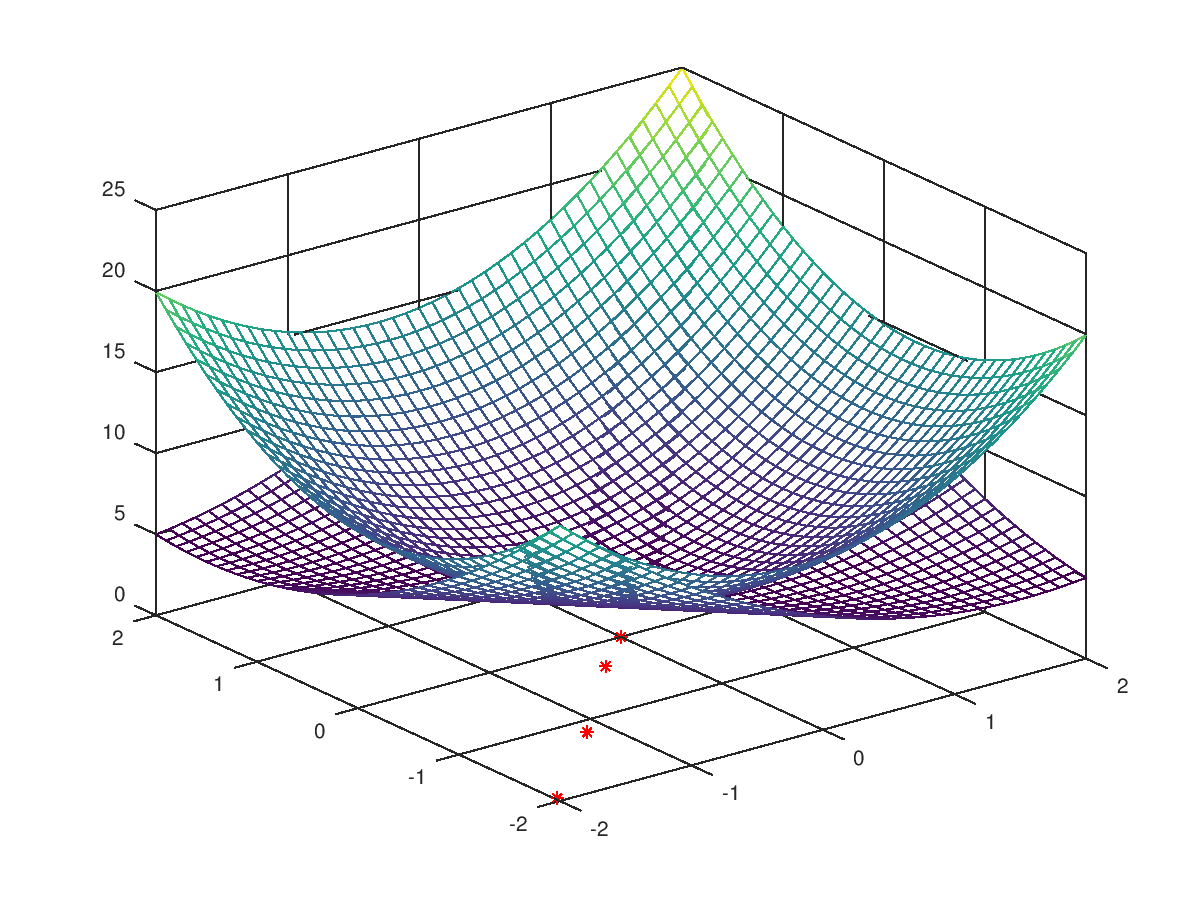
\includegraphics[width=150px]{images/poised_bad.png} }
        \item<3> The geometry can be measured by its $\Lambda$-poisedness
        \item<3> Constructing poised sets over ellipses is well known
        \item<3> Constraints limit what points are available for the sample set
    \end{itemize}
\end{frame}

\begin{frame}

\end{frame}


\section{Always Feasible Algorithm}


\begin{frame}{Feasible Derivative Free Algorithm Part 1}
    \begin{itemize}
        \item We experimented with several variations of an algorithm following the outline in ``Global convergence of trust region algorithms for convex constrained minimization without derivatives."
        \item This algorithm was promising after bench-marking our algorithms on the Hott-Schittowski problem set.
        \item The convergence analysis for this variant is promising
    \end{itemize}
\end{frame}


\begin{frame}{Feasible Derivative Free Algorithm Part 2}
    \begin{itemize}
        \item We define two trust regions:
        \begin{itemize}
            \item The inner trust region is used for constructing sample points
            \item The outer trust region is used as the search space for computing the next iterate
        \end{itemize}
        \item The inner trust region is chosen by maximizing the volume of an ellipsoid within the outer trust region intersect the constraints
        \item Even if the feasible region is narrow, the trust region is easy to optimize
    \end{itemize}
\end{frame}


\begin{frame}{}
\includegraphics[width=300px]{images/ellipse_at_current_iterate.png}
\end{frame}


\section{Convergence Analysis}

\frame {
\frametitle{Convergence Analysis}

\begin{itemize}
    \item Convergence relies on the results found in ``Global convergence of trust region algorithms for convex constrained minimization without derivatives."
    
    \item Two criteria must be satisfied:
    \begin{itemize}
        \item Efficiency: $$m_f^{(k)}(x^{(k)}) - m_f^{(k)}(x^{(k+1)}) \ge c_1 \xi^{(k)} \min \{\frac{\xi^{(k)}}{1 + \|\nabla^2 m_f^{(k)}(x^{(k)})\|}, \Delta_k, 1\}$$
        \item Accuracy: $$\|\nabla m_f^{(k)}(x^{(k)}) - \nabla f (x^{(k)})\| \le c_2 \Delta_k$$
    \end{itemize}
    \item The first of these can be satisfied using the Generalized Cauchy Point
\end{itemize}
}



\frame {
\frametitle{Linear Convergence Analysis}

\begin{itemize}
    \item In order to satisfy the accuracy condition, we must be able to show that we can always find a suitable ellipse.
    \item The ellipse must be feasible and have a bounded condition number in order to satsify the accuracy condition.
    \item We provide an algorithm for finding a feasible sphere, which is then used as input to a local search over ellipsoids to increase its volume
    \item If the current iterate does not have two or more active consntraints, this is easily done for linear constraints.
\end{itemize}
}


\frame {
\frametitle{General Convex algorithm}

\begin{itemize}
    \item With convex constraints, we still model the feasible region with linear constraints.
    \item We show that for a small enough trust region, we can still find a feasible ellipse.
    \item The ellipse we find may be much smaller than what is possible.
\end{itemize}

}


\frame {
\frametitle{General Convex algorithm}

\begin{itemize}
    \item We also experiment with other methods for computing a feasible ellipse.
    \item We also extend the problem of finding a maximal ellipsoid within a polyhedron, to the maximal ellispe within several special cones.
    \item Alternatively, we can add linear constraints that cut off any point that is found to be infeasible.
    \item We choose the linear constraint to remove the infeasible point to maximize the current lagrange polynomial within the resulting feasible region.
    \item We also consider kriging models of the constraints, as this allows an arbitrary number of points to be added.
\end{itemize}

}

\section{Future Work}

\frame{
\frametitle{Using Fewer Sample Points}
    \begin{itemize}
        \item With general convex constraints, sufficiently poised sets within the feasible region may not exist.
        \item To illustrate, consider finding a fully quadratic model in 2-dimensions.
        \item As the constraints become more thin,
            \begin{itemize}
                \item The model becomes less poised
                \item There is less need for requiring the model to be quadratic in $y$.
            \end{itemize}
        \item We would prefer to use a subset of all quadratics, with fewer points to approximate them.
    \end{itemize}
}

\frame {
\frametitle{2D Illustration}
    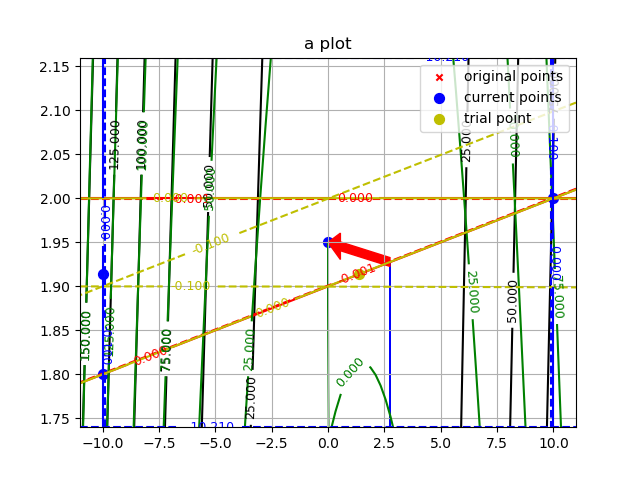
\includegraphics[width=150px]{images/2_2_4_68.png}
    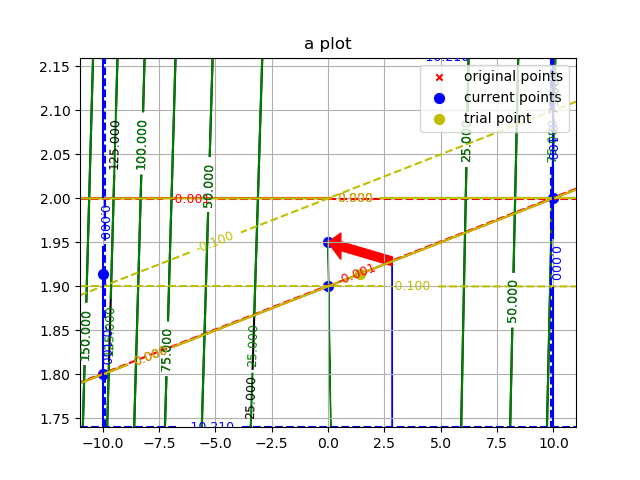
\includegraphics[width=150px]{images/2_3_5_1.png}
}

\frame {
\frametitle{Full pivoting}
    \begin{itemize}
        \item One approach is to use full pivoting within the LU factorization used compute the Lagrange polynomials.

        \item When there are no more pivots greater than a threshold, the LU factorization terminates, and only uses the points and polynomials already computed after zeroing the remaining entries.
        
        \item This method will provide the next point to use as well as the next polynomial to include.
        
    \end{itemize}
}

\frame {
\frametitle{Undetermined Coefficients}
    \begin{itemize}
        \item In [J. Belly, P.E. Belley, A.G.R. Day,. 2013], the authors develop an algorithm for approximating a subset of all partial derivatives
%         ``Multivariate polynomial interpolation and meshfree differentation via undetermined coefficients"

        \item For one dimensional problems, they provide a recursive formula for approximating the $\alpha$ derivative on a set of points $\sigma$:
\begin{math}
    L_f^{\alpha}(p; \sigma) = L_f^{\alpha}(p; \sigma \setminus p_m) + \big(f(p_m) - L_f(p_m; \sigma \setminus p_m)\big) l_m^{(\alpha)}(p; \sigma)
\end{math}
        
        \item In general, they use a method of undetermined coefficients to compute arbitrary partial derivatives in $n$-dimensions.
    \end{itemize}
}



\frame {
\frametitle{Including Function Values}
    \begin{itemize}
        \item There may be feasible directions where the constraints are not narrow, but the function does not change quickly.
        
        \item The error bounds in this paper as well as function values already computed may provide a way to choose a subset of points that reduces the error over the feasible region.

        \item This method uses not only the constraints, but existing function values to choose the next iterate.
    \end{itemize}
}

\color{red}
\frame {
\frametitle{Low hanging fruit}
    \begin{itemize}
        \item the current iterate need not be evaluated.
    \end{itemize}
}
\color{black}




\end{document}
